\documentclass[12pt, psamsfonts]{amsart}

%-------Packages---------
\usepackage{amssymb,amsfonts}
\usepackage{semantic}
\usepackage{fullpage}
\usepackage{tikz-cd}
\usepackage{todonotes}
\usepackage{physics}
\usepackage[all,arc]{xy}
\usepackage{enumerate}
\usepackage{enumitem}
\usepackage{mathrsfs}
\usepackage{theoremref}
\usepackage{graphicx}
\usepackage[bookmarks]{hyperref}

\usepackage{amsthm}
\makeatletter
\def\th@plain{%
  \thm@notefont{}% same as heading font
  \itshape % body font
}
\def\th@definition{%
  \thm@notefont{}% same as heading font
  \normalfont % body font
}
\makeatother

%--------Theorem Environments--------
%theoremstyle{plain} --- default
\newtheorem{thm}{Theorem}[subsection]
\newtheorem{cor}[thm]{Corollary}
\newtheorem{prop}[thm]{Proposition}
\newtheorem{lem}[thm]{Lemma}
\newtheorem{conj}[thm]{Conjecture}
\newtheorem{quest}[thm]{Question}

\theoremstyle{definition}
\newtheorem{defn}[thm]{Definition}
\newtheorem{defns}[thm]{Definitions}
\newtheorem{con}[thm]{Construction}
\newtheorem{exmp}[thm]{Example}
\newtheorem{exmps}[thm]{Examples}
\newtheorem{notn}[thm]{Notation}
\newtheorem{notns}[thm]{Notations}
\newtheorem{addm}[thm]{Addendum}
\newtheorem*{exer}{Exercise}

\theoremstyle{remark}
\newtheorem{rem}[thm]{Remark}
\newtheorem{rems}[thm]{Remarks}
\newtheorem{warn}[thm]{Warning}
\newtheorem{sch}[thm]{Scholium}

\makeatletter
\makeatother
\numberwithin{equation}{subsection}

\bibliographystyle{plain}

\begin{document}

\title{Stellar Consensus Protocol}
\author{Hidenori Shinohara}

\begin{abstract}
    This is my personal notes on the Stellar consensus protocol.
    This roughly follows the structure of the white paper on https://www.stellar.org/.
\end{abstract}

\maketitle

\tableofcontents

\section{Federated Byzantine Agreement System}

\subsection{Quorums}

\begin{defn}[Federated Byzantine Agreement System]
    Let $V$ be a set and $Q:V \rightarrow 2^{2^V} \setminus \{ \emptyset \}$ be a function such that $\forall v \in V, \forall q \in Q(v), v \in q$.
    Then we call the pair $\ev{V, Q}$ a federated Byzantine agreement system, or FBAS for short.
\end{defn}

\begin{rem}
    For each node $v$, $Q(v)$ is a set of subsets of $V$.
    For instance, node $v_1$ may trust $v_2, v_3, v_4$ and may have $Q(v_1) = \{ \{ v_1, v_2, v_3, v_4 \} \} \subset 2^V$.

    We explicitly exclude $\{ \emptyset \}$ from the co-domain because we want $Q(v) \ne \emptyset$ for all $v \in V$.
    This is necessary because if $Q(v) = \emptyset$ for some $v \in V$, it satisfies $\forall q \in Q(v), v \in q$.
\end{rem}

\begin{defn}[Quorum]
    Let $\ev{V, Q}$ be an FBAS\@.
    $U \subset V$ is called a quorum if and only if $U \ne \emptyset$ and $\forall v \in U, \exists q \in Q(v), q \subset U$.
\end{defn}

\begin{thm}\label{union_quorums}
    In an FBAS $\ev{V, Q}$, the union of two quorums is a quorum.
\end{thm}

\begin{proof}
    Let $U_1, U_2$ be two quorums.
    Let $v \in U_1 \cup U_2$.
    Then $v \in U_i$ for $i = 1$ or $i = 2$.
    Then $q \subset U_i$ for some $q \in Q(v)$.
    Therefore, $q \subset U_1 \cup U_2$, so $U_1 \cup U_2$ is indeed a quorum.
\end{proof}

\begin{cor}
    The set of quorums of a given FBAS is closed under union.
\end{cor}

\begin{thm}
    In an FBAS $\ev{V, Q}$, $V$ is a quorum.
\end{thm}

\begin{proof}
    For any $v \in V$, for any $q \in Q(v)$, $q \subset V$.
    Therefore, $V$ is indeed a quorum.
\end{proof}

\begin{exmp}
    One might wonder if the intersubsection of quorums is always a quorum.
    However, this is not true in general.

    Let $V = \{ v_1, \ldots, v_4 \}$ and
    \begin{itemize}
        \item
            $Q(v_1) = \{ \{ v_1, v_2, v_3 \}, \{ v_1, v_2, v_4 \}, \{ v_1, v_3, v_4 \} \}$,
        \item
            $\vdots$
        \item
            $Q(v_4) = \{ \{ v_1, v_2, v_4 \}, \{ v_1, v_3, v_4 \}, \{ v_2, v_3, v_4 \} \}$.
    \end{itemize}

    In other words, $Q(v_i) = \{ U \subset V \mid \abs{U} = 3, v_i \in U \}$.

    Then $U_1 = \{ v_1, v_2, v_3 \}$ is a quorum, and $U_2 = \{ v_2, v_3, v_4 \}$ is a quorum.
    However, $U_1 \cap U_2 = \{ v_2, v_3 \}$ is not a quorum because the size of any quorum slice is 3.
\end{exmp}

\begin{defn}[Quorum Intersubsection]
    Let $\ev{V, Q}$ be an FBAS\@.
    We say $\ev{V, Q}$ enjoys quorum intersubsection if and only if for any pair of quorums $U_1, U_2$, $U_1 \cap U_2 \ne \emptyset$.
\end{defn}

\begin{defn}[Delete]\label{delete_fbas}
    Let $\ev{V, Q}$ be an FBAS and $B \subset V$.
    Then the FBAS $\ev{V, Q}^B$ is defined to be $\ev{V \setminus B, Q^B}$ where $\forall v \in V \setminus B, Q^B(v) = \{ q \setminus B \mid q \in Q(v) \}$.
\end{defn}

\begin{rem}
    One may think that this is related to fail-stop behaviors where $B$ is the set of nodes that stopped responding.
    In general, however, this is not true as we also remove nodes from quorum slices.
    One can think of this as the alternate universe where nodes from $B$ simply did not even exist from the beginning.
\end{rem}

\begin{thm}
    Definition~\ref{delete_fbas} is well-defined.
    In other words, if $\ev{V, Q}$ is an FBAS and $B \subset V$, then $\ev{V, Q}^B$ is an FBAS\@.
\end{thm}

\begin{proof}
    Let $v \in V \setminus B, q' \in Q^B(v)$ be given.
    Then $q' = q \setminus B$ for some $q \in Q(v)$.
    By the definition of an FBAS, $v \in q$.
    Since $v \notin B$, $v \in q \setminus B = q'$.
    Therefore, $\ev{V, Q}^B$ is an FBAS\@.
\end{proof}

\begin{thm}\label{quorum_delete_fbas}
    Let $U$ be a quorum in FBAS $\ev{V, Q}$, let $B \subset V$ be a set of nodes, and let $U' = U \setminus B$.
    If $U' \ne \emptyset$, then $U'$ is a quorum in $\ev{V, Q}^B$.
\end{thm}

\begin{proof}
    Since $U' \ne \emptyset$, it suffices to show that $\forall v \in U', \exists q \in Q^B(v), q \subset U'$.
    Let $v \in U'$.
    Then $v \in U$.
    Since $U$ is a quorum in $\ev{V, Q}$, we can find $q \in Q(v)$ such that $q \subset U$.
    Then $q' = q \setminus B \in Q^B(v)$, and $q' = q \setminus B \subset U \setminus B = U'$.
    Therefore, $U'$ is a quorum in $\ev{V, Q}^B$.
\end{proof}

\begin{rem}
    One can think of this theorem as ``\textit{A quorum in the `original' universe is a quorum in the `alternate' universe.}"
\end{rem}

\begin{defn}[Quorum Intersubsection Despite $B$]
    Let $\ev{V, Q}$ be an FBAS and $B \subset V$ be a set of nodes.
    We say $\ev{V, Q}$ enjoys quorum intersubsection despite $B$ if and only if $\ev{V, Q}^B$ enjoys quorum intersubsection.
\end{defn}

\begin{rem}
    Quorum intersubsection despite $B$ is related to system-level safety when nodes in $B$ act arbitrarily.
    For instance, suppose $\ev{V, Q}$ is an FBAS, $B$ is the set of all ill-behaved nodes, and $\ev{V, Q}$ enjoys quorum intersubsection despite $B$.
    Suppose two well-behaved nodes $v_1, v_2$ agree with contradictory statements $a_1, a_2$ in quorums $q_1, q_2$, respectively.
    Then $q_1 \cap q_2 \ne \emptyset$ have well-behaved nodes who agreed with both $a_1$ and $a_2$.
    This is a contradiction because a well-behaved node cannot contradict itself.
    This example illustrates how the concept of quorum intersubsection despite $B$ is related to system-level safety when nodes in $B$ experience Byzantine failures.
\end{rem}

\begin{defn}[Quorum Availability Despite $B$]\label{def_quorum_availability}
    Let $\ev{V, Q}$ be an FBAS and $B \subset V$ be a set of nodes.
    We say $\ev{V, Q}$ enjoys quorum availability despite $B$ if and only if $V \setminus B$ is a quorum in $\ev{V, Q}$ or $B = V$.
\end{defn}

\begin{thm}\label{quorum_availability_equivalence_condition}
    Let $\ev{V, Q}$ be an FBAS and $B \subset V$.
    $\ev{V, Q}$ enjoys quorum availability despite $B$ if and only if $\forall v \in V \setminus B$, there exists a quorum $U_v$ such that $v \in U_v \subset (V \setminus B)$.
\end{thm}

\begin{proof}
    If $V = B$, we are done.
    Suppose otherwise.
    \begin{align*}
        \forall v \in V \setminus B, \exists \text{a quorum $U_v$}, v \in U_v \subset (V \setminus B)
            &\implies \bigcup_{v \in V \setminus B} U_v \text{ is a quorum in $\ev{V, Q}$} \\
            &\implies \text{$V \setminus B$ is a quorum in $\ev{V, Q}$}
    \end{align*}
    by Theorem~\ref{union_quorums}.
    On the other hand, if $V \setminus B$ is a quorum in $\ev{V, Q}$, then $\forall v \in V \setminus B, \exists \text{a quorum $U_v$}, v \in U_v \subset (V \setminus B)$ because we can let $U_v = V \setminus B$ for each $v$.
\end{proof}

\begin{rem}
    Theorem~\ref{quorum_availability_equivalence_condition} shows that $\ev{V, Q}$ enjoys quorum availability despite $B$ if all nodes in $V \setminus B$ can find a quorum without $B$.
    This is related to the liveness of the system.
    If $\ev{V, Q}$ enjoys quorum availability despite $B$, then regardless of what happens to nodes in $B$, nodes in $V \setminus B$ can keep going.
\end{rem}

\begin{defn}[$v$-blocking]\label{def_v_blocking}
    Let $\ev{V, Q}$ be an FBAS\@.
    Let $v \in V$.
    A subset $B \subset V$ is called $v$-blocking if and only if $\forall q \in Q(v), q \cap B \ne \emptyset$.
\end{defn}

\begin{rem}
    Intuitively, if a subset $B \subset V$ is $v$-blocking, then one may think of it as ``\textit{$v$ can't really get by without $B$}."
    The following theorem can be interpreted as ``\textit{If $v$ can't get by without $B$, $v$ can't get by without $C$ for any $C \supset B$}."
\end{rem}

\begin{thm}\label{basic_prop_v_blocking}
    Let $\ev{V, Q}$ be an FBAS\@.
    Let $v \in V$.
    Then
    \begin{itemize}
        \item
            The union of two $v$-blocking sets is $v$-blocking.
        \item
            Any superset of a $v$-blocking set is $v$-blocking.
    \end{itemize}
\end{thm}

\begin{proof}
    It suffices to only prove the second statement.
    If $B \subset B'$ and $B$ is $v$-blocking, $q \cap B' \supset q \cap B \ne \emptyset$ for any $q \in Q(v)$.
\end{proof}

\begin{thm}\label{v_blocking_delete}
    Let $\ev{V, Q}$ be an FBAS\@.
    Let $A \subsetneq V$ and $U_1, U_2$ be a partition of $V \setminus A$.
    Let $v \in U_1$.
    If $U_2$ is not $v$-blocking in $\ev{V, Q}$, then $U_2$ is not $v$-blocking in $\ev{V, Q}^A$.
\end{thm}

\begin{proof}
    Since $U_2$ is not $v$-blocking in $\ev{V, Q}$, there exists $q_v \in Q(v)$ such that $q_v \cap U_2 = \emptyset$.
    \begin{align*}
        (q_v \setminus A) \cap U_2
            &= (q_v \cap U_2) \setminus (A \cap U_2) \\
            &= q_v \cap U_2 = \emptyset.
    \end{align*}
    Thus $U_2$ is not $v$-blocking in $\ev{V, Q}^A$.
\end{proof}

\begin{thm}\label{quorum_availability_v_blocking}
    Let $\ev{V, Q}$ be an FBAS\@.
    Let $B \subset V$.
    $\ev{V, Q}$ enjoys quorum availability despite $B$ if and only if $B$ is not $v$-blocking for any $v \in V \setminus B$.
\end{thm}

\begin{proof}
    \begin{align*}
        \forall v \in V \setminus B, \neg(\text{$B$ is $v$-blocking})
            &\iff \forall v \in V \setminus B, \neg(\forall q \in Q(v), q \cap B \ne \emptyset) \\
            &\iff \forall v \in V \setminus B, \exists q \in Q(v), q \cap B = \emptyset \\
            &\iff \forall v \in V \setminus B, \exists q \in Q(v), q \subset V \setminus B \\
            &\iff \text{$V = B$ or $V \setminus B$ is a quorum in $\ev{V, Q}$} \\
            &\iff \text{$\ev{V, Q}$ enjoys quorum availability despite $B$}
    \end{align*}
\end{proof}

\subsection{Dispensable Sets}

\begin{defn}[Dispensable Set]\label{def_dset}
    Let $\ev{V, Q}$ be an FBAS and $B \subset V$ be a set of nodes.
    $B$ is called a dispensable set, or DSet, if and only if $\ev{V, Q}$ enjoys both quorum intersubsection despite $B$ and quorum availability despite $B$.
\end{defn}

\begin{defn}[Intact and Befouled]\label{def_intact_befouled}
    Let $\ev{V, Q}$ be an FBAS and $v \in V$.
    $v$ is said to be intact if and only if there exists a DSet $B$ containing all ill-behaved nodes and $v \notin B$.
    $v$ is said to be befouled if and only if $v$ is not intact.
\end{defn}

\begin{figure}[!htb]
    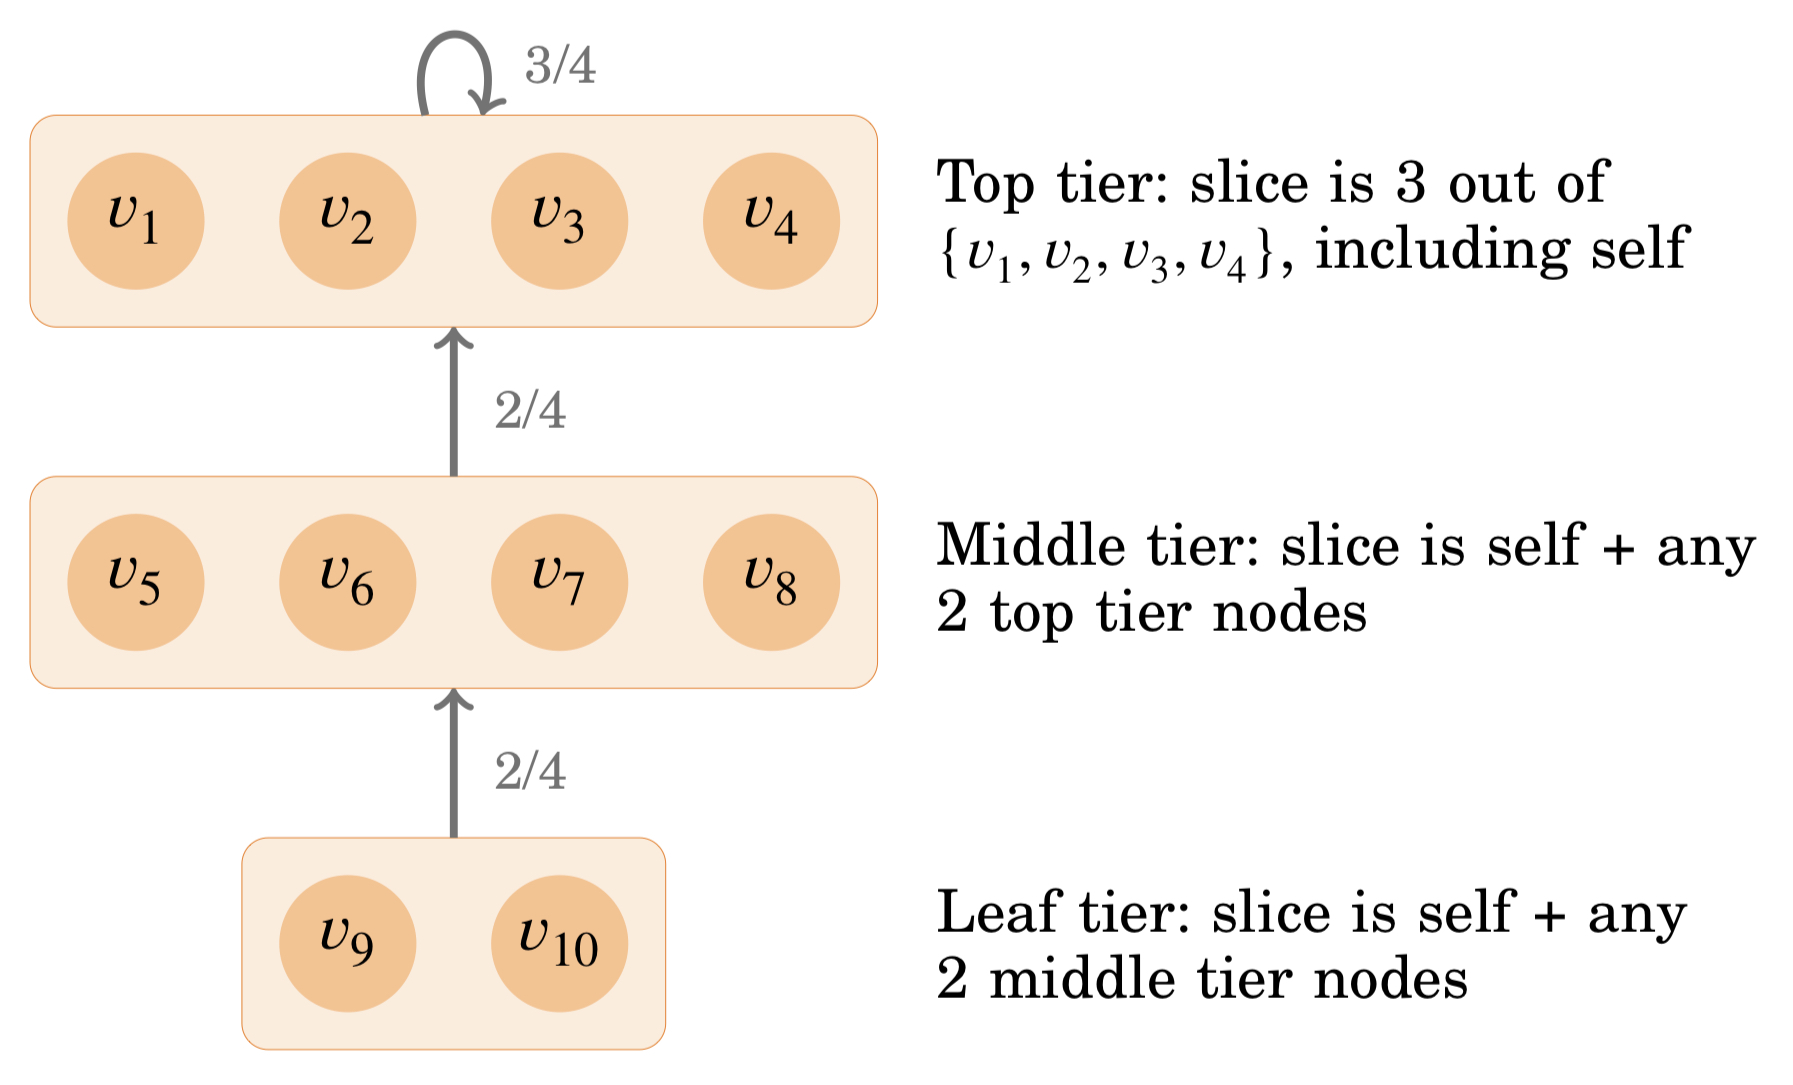
\includegraphics[width=.5\linewidth]{img/tiered_quorum_example.jpeg}
        \caption{Tiered Quroum Example (P.5 of the white paper)}
    \label{fig:tiered_quorum_example}
\end{figure}

\begin{exmp}
    We will use Figure~\ref{fig:tiered_quorum_example} as an example.

    \begin{itemize}
        \item
            The smallest DSet containing $v_5, v_6$ in Figure~\ref{fig:tiered_quorum_example} is $\{ v_5, v_6, v_9, v_{10} \}$.
            \begin{itemize}
                \item
                    First, we will show that $B = \{ v_5, v_6 \}$ is not a DSet.
                    By definition,
                    \begin{align*}
                        Q^B(v_9) &= \{ \{ v_9 \}, \{ v_9, v_7 \}, \{ v_9, v_8 \}, \{ v_9, v_7, v_8 \} \} \\
                        Q^B(v_{10}) &= \{ \{ v_{10} \}, \{ v_{10}, v_7 \}, \{ v_{10}, v_8 \}, \{ v_{10}, v_7, v_8 \} \}
                    \end{align*}
                    This implies that $U_9 = \{ v_9 \}$ and $U_{10} = \{ v_{10} \}$ are both quorums.
                    Then $U_9 \cap U_{10} = \emptyset$, so $\ev{V, Q}^B$ does not enjoy quorum intersubsection.
                    Therefore, $B$ is not a DSet.

                    Next, we will consider $C = \{ v_5, v_6, v_1 \}$.
                    Then we can use the same argument as above.
                    $U_9 = \{ v_9 \} \in Q^C(v_9)$ and $U_{10} = \{ v_{10} \} \in Q^C(v_{10})$, and the intersubsection is empty.
                    Therefore, $C$ is not a DSet.
                    It is easy to see that this argument works for the case of $\{ v_5, v_6, v_i \}$ for any $i = 1, 2, 3, 4$.

                    We will consider $D = \{ v_5, v_6, v_9 \}$.
                    Similarly, $U = \{ v_{10} \} \in Q^D(v_{10})$ is a quorum.
                    Moreover, $U' = \{ v_1, v_2, v_3, v_4 \}$ is a quorum.
                    Then $U \cap U' = \emptyset$, so $\ev{V, Q}^D$ does not enjoy quorum intersubsection.
                    It is easy to see that a similar argument shows that $\{ v_5, v_6, v_{10} \}$ is not a DSet.

                    Finally, we will show that $E = \{ v_5, v_6, v_9, v_{10} \}$ is a DSet.
                    $V \setminus E$ is a quorum in $\ev{V, Q}$ because every node in $V \setminus E$ has a quorum slice consisting of nodes in $V \setminus E$.
                    If a quorum in $\ev{V, Q}^E$ contains $v_7$ or $v_8$, then it must contain some of $v_1, v_2, v_3, v_4$.
                    If a quorum in $\ev{V, Q}^E$ contains at least one of $v_1, v_2, v_3$, or $v_4$, then it must contain at least three of $v_1, v_2, v_3, v_4$.
                    Therefore, any intersubsection of two quorums in $\ev{V, Q}^E$ contains at least two of $v_1, v_2, v_3, v_4$ by the pigeon hole principle.

                    Therefore, $E$ is indeed a smallest DSet containing $v_5$ and $v_6$.
                \item
                    We showed that $B = \{ v_5, v_6 \}$ is not a DSet because $\ev{V, Q}$ does not enjoy quorum intersubsection despite $B$.
                    What this means is that if both $v_5$ and $v_6$ either stop responding or are malicious, then it is not possible to guarantee safety for $v_9$ and $v_{10}$.
                    For instance, consider the following situation:
                    \begin{itemize}
                        \item
                            Both $v_5$ and $v_6$ tell $v_9$ and $v_{10}$ that $Q(v_5) = Q(v_6) = \{ \{ v_5, v_6 \} \}$ convincing that $\{ v_5, v_6, v_9 \}$ and $\{ v_5, v_6, v_{10} \}$ are both quorums.
                        \item
                            Both $v_5$ and $v_6$ tell $v_9$ that they want to process a certain transaction.
                            This transaction does not contradict what $v_9$ knows about $v_5$.
                            Moreover, everyone in the quorum $\{ v_5, v_6, v_9 \}$ is in favor of this transaction.
                            Thus there is no reason for $v_9$ to not believe this transaction.
                        \item
                            Both $v_5$ and $v_6$ tell $v_{10}$ that they want to process a certain transaction that contradicts the transaction they told $v_5$ about.
                            For the same reason, there is no reason for $v_{10}$ to not believe this transaction.
                        \item
                            Then the network processes contradicting transactions.
                            This can let $v_5$ double-spend some money, for instance.
                        \item
                            One can verify that this is possible by looking into the definition of accepting, confirming and such that are introduced in later chapters.
                    \end{itemize}
            \end{itemize}
        \item
            $B = \{ v_1 \}$ is a DSet.
            \begin{itemize}
                \item
                    First, we will check if $\ev{V, Q}$ enjoys quorum intersubsection despite $B$.

                    Consider $\ev{V, Q}^B$.
                    Any quorum containing $v_9$ and/or $v_{10}$ must contain at least two of $v_5, v_6, v_7, v_8$.
                    Any quorum containing at least one of $v_5, \cdots, v_8$ must contain at least one of $v_2, v_3, v_4$.
                    Any quorum containing at least one of $v_2, v_3, v_4$ must contain at least two of $v_2, v_3, v_4$.
                    This is because $Q(v_i)^B = \{ \{ v_2, v_3, v_4 \}, \{ v_i, v_j \}, \{ v_i, v_k \} \}$ where $\{ i, j, k \} = \{ 2, 3, 4 \}$.

                    Therefore, the intersubsection of any two quorums must contain at least one of $v_2, v_3, v_4$ by the pigeon hole principle.

                    Next, we need to check if $\ev{V, Q}$ enjoys quorum availability despite $B$.
                    $V \setminus B$ is indeed a quorum in $\ev{V, Q}$ because each node in $V \setminus B$ has a quorum slice that does not contain $v_1$.
                \item
                    We showed that $B$ is indeed a DSet.
                    What this means is that even if $v_1$ stops responding or becomes malicious, the rest of the network can make progress safely.
                    For instance, suppose that $v_1$ becomes malicious and tries to double-spend money.
                    $v_1$ might tell $v_5$ that it wants to process a certain transaction.
                    Similarly, $v_1$ might tell $v_6$ that it wants to process a contradicting transaction.
                    However, every quorum slice of $v_5$ and $v_6$ contains at least one tier-1 node that is not $v_1$.
                    Suppose that $v_5$ asks $v_2$ what it thinks, and $v_6$ asks $v_3$ what it thinks.
                    Then every quorum slice of $v_2$ and $v_3$ contains 3 tier-1 nodes.
                    By the pigeon hole principle, at least one tier-1 node that is not $v_1$ gets asked what it thinks about the contradicting transactions from $v_5$.
                    The tier-1 node does not agree with them and $v_1$'s attempt to double-spend money fails.
            \end{itemize}
    \end{itemize}
\end{exmp}

\begin{thm}\label{intersubsection_dset}
    If $B_1$ and $B_2$ are DSets in an FBAS $\ev{V, Q}$ enjoying quorum intersubsection, then $B = B_1 \cap B_2$ is a DSet, too.
\end{thm}

\begin{proof}
	If $B_1 = V$ or $B_2 = V$, then we are done.
	Suppose otherwise.

    First, we will show that $\ev{V, Q}$ enjoys quorum availability despite $B$.
    By Definition~\ref{def_quorum_availability}, it suffices to show that $V = B$ or $V \setminus B$ is a quorum in $\ev{V, Q}$.
    Since we assumed that $B_1 \ne V$ and $B_2 \ne V$, $B \ne V$.
    Therefore, we will show that $V \setminus B$ is a quorum in $\ev{V, Q}$.
    By basic set theory, $V \setminus B = V \setminus (B_1 \cap B_2) = (V \setminus B_1) \cup (V \setminus B_2)$.
    Since $B_1$ is a DSet, $V = B_1$ or $V \setminus B_1$ is a quorum in $\ev{V, Q}$.
    Since we assumed that $V \ne B_1$ earlier, $V \setminus B_1$ is a quorum in $\ev{V, Q}$.
    Similarly, $V \setminus B_2$ is a quorum in $\ev{V, Q}$.
    By Theorem~\ref{union_quorums}, the union $(V \setminus B_1) \cup (V \setminus B_2) = V \setminus B$ is a quorum in $\ev{V, Q}$.

    Next, we will show that $\ev{V, Q}$ enjoys quorum intersubsection despite $B$.
	Let $U_a, U_b$ be quorums in $\ev{V, Q}^B$.
    We want to show that $U_a \cap U_b \ne \emptyset$.
    We will do so by proving a stronger statement, which is $(U_a \cap U_b) \setminus B_1 \ne \emptyset$.
    In other words, we will show that $(U_a \setminus B_1) \cap (U_b \setminus B_1) \ne \emptyset$.

    Since $B_1$ is a DSet, $\ev{V, Q}$ enjoys quorum intersubsection despite $B_1$.
    In other words, $\ev{V, Q}^{B_1}$ enjoys quorum intersubsection.
    Therefore, it suffices to show that $U_a \setminus B_1$ and $U_b \setminus B_1$ are both quorums in $\ev{V, Q}^{B_1}$.
    By Theorem~\ref{quorum_delete_fbas}, $U_a \setminus B_1$ and $U_b \setminus B_1$ are quorums in $(\ev{V, Q}^B)^{B_1}$ if $U_a \setminus B_1 \ne \emptyset$ and $U_b \setminus B_1 \ne \emptyset$.
    Since $(\ev{V, Q}^B)^{B_1} = \ev{V, Q}^{B_1}$, it suffices to show that $U_a \setminus B_1 \ne \emptyset$ and $U_b \setminus B_1 \ne \emptyset$.
    
    We will first show that $U_a \setminus B_1 \ne \emptyset$.
    By basic set theory,
	\begin{align*}
        U_a &= U_a \setminus B \\
            &= U_a \setminus (B_1 \cap B_2) \\
            &= (U_a \setminus B_1) \cup (U_a \setminus B_2)
	\end{align*}
	because $U_a \cap B = \emptyset$.

	This implies that $(U_a \setminus B_1) \cup (U_a \setminus B_2) \ne \emptyset$.
    If $U_a \setminus B_1$ is nonempty, we are done.
    Suppose $U_a \setminus B_2$ is nonempty.
    We will show that this implies that $U_a \setminus B_1 \ne \emptyset$.
    We will do so by first finding two quorums in $\ev{V, Q}^{B_2}$ whose intersubsection is a subset of $U_a \setminus B_1$.
	Since $\ev{V, Q}^{B_2}$ enjoys quorum intersubsection, the intersubsection of such two quorums must be nonempty, which in turn shows that $U_a \setminus B_1$ is nonempty.

	\begin{itemize}
		\item
            We claim that $U_a \setminus B_2$ is a quorum in $\ev{V, Q}^{B_2}$.
            $U_a$ is a quorum in $\ev{V, Q}^B$.
            Since $U_a \setminus B_2$ is assumed to be nonempty, $U_a \setminus B_2$ is a quorum in $(\ev{V, Q}^B)^{B_2}$ by Theorem~\ref{quorum_delete_fbas}.
            Since $(\ev{V, Q}^B)^{B_2} = \ev{V, Q}^{B_2}$, $U_a \setminus B_2$ is a quorum in $\ev{V, Q}^{B_2}$.
		\item
            $V \setminus B_2 \ne \emptyset$ is a quorum in $\ev{V, Q}$ because $\ev{V, Q}$ must enjoy quorum availability despite $B_2$ and $B_2 \ne V$.
			Similarly, $V \setminus B_1 \ne \emptyset$ is a quorum in $\ev{V, Q}$.
			Because $\ev{V, Q}$ enjoys quorum intersubsection, $(V \setminus B_1) \cap (V \setminus B_2) \ne \emptyset$.
			In other words, $(V \setminus B_1) \setminus B_2 \ne \emptyset$.
            By applying Theorem~\ref{quorum_delete_fbas} to the fact that $V \setminus B_1$ is a quorum in $\ev{V, Q}$ and $(V \setminus B_1) \setminus B_2 \ne \emptyset$, we can conclude that $(V \setminus B_1) \setminus B_2$ is a quorum in $\ev{V, Q}^{B_2}$.
	\end{itemize}
	Since $\ev{V, Q}^{B_2}$ enjoys quorum intersubsection, $(U_a \setminus B_2) \cap ((V \setminus B_1) \setminus B_2) \ne \emptyset$.
	\begin{align*}
        \emptyset
            &\ne (U_a \setminus B_2) \cap ((V \setminus B_1) \setminus B_2) \\
            &= (U_a \cap (V \setminus B_1)) \setminus B_2 \\
            &\subset U_a \cap (V \setminus B_1) \\
            &= U_a \setminus B_1.
	\end{align*}
	Thus, $U_a \setminus B_1 \ne \emptyset$.

	The same argument will show that $U_b \setminus B_1 \ne \emptyset$.
\end{proof}

\begin{rem}
    Theorem~\ref{intersubsection_dset} states that the intersubsection of two DSets is a DSet if the FBAS enjoys quorum intersubsection.
    One might wonder if the union of two DSets is a DSet when the FBAS enjoys quorum intersubsection.
    However, this is not true in general.
    Consider the FBAS $\ev{V, Q}$ where $V = \{ v_1, v_2, v_3, v_4 \}$ and $Q(v_i) = \{ U \subset V \mid v_i \in U, \abs{U} = 3 \}$.
    This FBAS enjoys quorum intersubsection by the pigeon-hole principle because each quorum contains at least 3 elements.
    Then $B = \{ v_1 \}$ is a DSet because
    \begin{itemize}
        \item
            Quorum intersubsection despite $B$
            \begin{itemize}
                \item
                    Every quorum slice in $\ev{V, Q}^B$ contains at least 2 nodes because every quorum slice in $\ev{V, Q}$ contains exactly 3 nodes.
                    This implies that any quorum in $\ev{V, Q}^B$ must contain at least 2 nodes.
                    By the pigeon-hole principle, every pair of quorums in $\ev{V, Q}^B$ must intersect.
            \end{itemize}
        \item
            Quorum availability despite $B$
            \begin{itemize}
                \item
                    $V \setminus B = \{ v_2, v_3, v_4 \}$ is a quorum in $\ev{V, Q}$ because $\{ v_2, v_3, v_4 \} \in Q(v_i)$ for each $i = 2, 3, 4$.
            \end{itemize}
    \end{itemize}
    Similarly, $C = \{ v_2 \}$ is a DSet.
    However, $B \cup C = \{ v_1, v_2 \}$ is not a DSet because $B \cup C \ne V$ and $V \setminus (B \cup C) = \{ v_3, v_4 \}$ is not a quorum in $\ev{V, Q}$.
\end{rem}

\begin{thm}\label{befouled_dset}
	In an FBAS with quorum intersubsection, the set of befouled nodes is a DSet.
\end{thm}

\begin{proof}
	Let $\ev{V, Q}$ be an FBAS with quorum intersubsection.
	Let $B$ be the intersubsection of all DSets that contain all ill-behaved nodes.
    We will show that $B$ is the set of befouled nodes by showing that $V \setminus B$ is the set of intact nodes.

    \begin{align*}
        v \in V \setminus B
            &\iff v \notin B \\
            &\iff \text{$\exists$ DSet $B_v$ that contains all ill-behaved nodes and $v \notin B_v$} \\
            &\iff \text{$v$ is intact}
    \end{align*}

	Therefore, $V \setminus B$ is precisely the set of intact nodes, and thus $B$ is the set of befouled nodes.

	By applying Theorem~\ref{intersubsection_dset} repeatedly, we can conclude that $B$ is a DSet.
\end{proof}

\begin{thm}\label{dset_v_blocking}
    Let $\ev{V, Q}$ be an FBAS and let $B \subset V$ be the set of befouled nodes.
    If $B$ is a DSet, $B$ is not $v$-blocking for any intact $v$.
\end{thm}

\begin{proof}
    By Definition~\ref{def_intact_befouled}, a node $v \in V$ is intact if and only if $v \notin B$.
    By Theorem~\ref{quorum_availability_v_blocking}, $\ev{V, Q}$ enjoys quorum availability despite $B$ if and only if $B$ is not $v$-blocking for any $v \in V \setminus B$.
    Since $B$ is a DSet, $\ev{V, Q}$ enjoys quorum availability despite $B$.
    Thus $B$ is not $v$-blocking for any intact $v$.
\end{proof}
\subsection{Voting, Accepting, and Ratifying}

The definitions of voting and accepting have a circular dependency.

\begin{defn}[Vote]\label{def_vote}
    A node $v$ votes for a statement $a$ if and only if $v$ asserts
    \begin{itemize}
        \item
            $a$ is valid,
        \item
            $a$ is consistent with all statements $v$ has accepted,
        \item
            $v$ has never voted against $a$,
        \item
            $v$ promises never to vote against $a$ in the future.
    \end{itemize}
\end{defn}

\begin{defn}[Accept]\label{def_accept}
    Let $\ev{V, Q}$ be an FBAS\@, and let $v \in V$.
    $v$ accepts a statement $a$ if and only if 
    \begin{itemize}
        \item
            It has never accepted a statement contradicting $a$.
        \item
            It determines that either
            \begin{itemize}
                \item
                    There exists a quorum $U$ such that $v \in U$ and each member of $U$ either voted for $a$ or broadcast that it has accepted $a$, or
                \item
                    There exists a $v$-blocking set $B$ such that every member of $B$ broadcast that it has accepted $a$.
            \end{itemize}
    \end{itemize}
\end{defn}

Note that it is possible for a node to accept a statement it did not vote for.
Furthermore, it is possible for a node to accept a statement after voting for a contradictory statement.

\begin{defn}[Ratify]\label{def_ratify}
    A quorum $U_a$ ratifies a statement $a$ if and only if every member of $U_a$ votes for $a$.
    A node $v$ ratifies $a$ if and only if $v$ is a member of a quorum $U_a$ that ratifies $a$.
\end{defn}

\begin{thm}\label{ratify_implies_accept}
    Let $\ev{V, Q}$ be an FBAS\@.
    If a node $v \in V$ ratifies a statement $a$, then it must accept $a$.
\end{thm}

\begin{proof}
    If a node $v$ ratifies $a$, then it is a member of a quorum $U \subset V$ that ratifies $a$.
    Thus every member of $U$ votes for $a$.
    This implies that $v$ also votes for $a$.
    By Definition~\ref{def_vote}, $v$ has never accepted a statement contradicting $a$.
    By Definition~\ref{def_accept}, $v$ accepts $a$.
\end{proof}

\begin{rem}
    Theorem~\ref{ratify_implies_accept} shows that ratifying is a stronger condition than accepting.
\end{rem}

\begin{thm}
    If an FBAS enjoys quorum intersubsection and contains no ill-behaved node, then two contradictory statements cannot be both ratified.
\end{thm}

\begin{proof}
    Suppose the statement is false and let $a, \bar{a}$ denote two contradictory statements ratified in such an FBAS\@.
    Let $U_a, U_{\bar{a}}$ denote quorums ratifying such statements, respectively.
    By the definition of quorum intersubsection, $U_a \cap U_{\bar{a}} \ne \emptyset$.
    Let $v \in U_a \cap U_{\bar{a}}$.
    This implies that $v$ voted for both $a$ and $\bar{a}$.
    However, this goes against the definition of voting.
    In other words, $v$ must be ill-behaved, which is a contradiction to our assumption.
\end{proof}

\begin{thm}\label{ill_behaved_ratify}
    Let $\ev{V, Q}$ be an FBAS\@.
    Let $B \subsetneq V$ be a subset containing all the ill-behaved nodes and suppose that $\ev{V, Q}^B$ enjoys quorum intersubsection.
    Let $v_1 \ne v_2 \in V \setminus B$.
    If $v_1$ ratifies a statement $a$, then $v_2$ cannot ratify any statement that contradicts $a$.
\end{thm}

\begin{proof}
    Suppose that the theorem is false and let $U_1, U_2$ be quorums of $v_1, v_2$ that ratify $a, \bar{a}$, respectively where $a$ and $\bar{a}$ are contradictory.
    Since $v_1 \in U_1 \setminus B$,  $U_1 \setminus B \ne \emptyset$.
    By Theorem~\ref{quorum_delete_fbas}, $U_1' = U_1 \setminus B$ is a quorum in $\ev{V, Q}^B$.
    Similarly, $U_2' = U_2 \setminus B$ is a quorum in $\ev{V, Q}^B$.
    Since $\ev{V, Q}^B$ enjoys quorum intersubsection, $U_1' \cap U_2' \ne \emptyset$.
    Let $v \in U_1' \cap U_2'$.
    Then $v \in U_1 \cap U_2$.
    In order for $U_1, U_2$ to ratify $a, \bar{a}$, respectively, $v$ must vote for both $a$ and $\bar{a}$.
    However, this is against the definition of voting.
    $v$ must be an ill-behaved node, so $v \in B$, which is a contradiction because $v \in U_1' \cap U_2' \subset U_1' = U_1 \setminus B$ where $B$ contains all ill-behaved nodes.
\end{proof}

\begin{thm}\label{intact_ratify_contradictory}
    Let $\ev{V, Q}$ be an FBAS with quorum intersubsection.
    Then two intact nodes in $V$ cannot ratify contradictory statements.
\end{thm}

\begin{proof}
    Let $v \ne v'$ be two intact nodes in $V$.
    Let $B \subset V$ be the set of befouled nodes.
    Then $v \notin B$ and $v' \notin B$.
    Since $\ev{V, Q}$ is an FBAS with quorum intersubsection, $B$ is a DSet by Theorem~\ref{befouled_dset}.
    By the definition of a DSet (Definition~\ref{def_dset}), $\ev{V, Q}^B$ enjoys quorum intersubsection.
    By Theorem~\ref{ill_behaved_ratify}, $v, v'$ cannot ratify contradictory statements.
\end{proof}

\begin{lem}\label{lem_intact_ratify}
    Let $\ev{V, Q}$ be an FBAS enjoying quorum intersubsection and $B$ be the set of befouled nodes.
    If $a$ is accepted by an intact node in $V$, then $a$ is ratified by some intact node in $\ev{V, Q}^B$.
\end{lem}

\begin{proof}
    Suppose that $a$ is accepted by one or more intact nodes in $V$.
    Since $V$ is finite, there has to be an intact node $v$ such that no intact nodes in $V$ accepted $a$ before $v$.

    By the definition of accepting(Definition~\ref{def_accept}), the moment $v$ accepted $a$, either
    \begin{itemize}
        \item
            there was a quorum $U$ of $v$ such that every element of $U$ either voted for $a$ or broadcast that it has accepted $a$, or
        \item
            there existed a $v$-blocking set such that every element in it broadcast that it has accepted $a$.
    \end{itemize}
    We claim that it could not have been the second one.
    On the contrary, suppose that it was the second one.
    Since no intact nodes in $V$ accepted $a$ before $v$, such a $v$-blocking set must have only had befouled nodes.
    Therefore, such a $v$-blocking set must be a subset of $B$.
    Since $\ev{V, Q}$ enjoys quorum intersubsection, $B$ is a DSet by Theorem~\ref{befouled_dset}.
    By Theorem~\ref{dset_v_blocking}, $B$ is not $v$-blocking.
    By taking the contrapositive of Theorem~\ref{basic_prop_v_blocking}, we conclude that no subset of $B$ is $v$-blocking.

    Therefore, it must have been the first case.
    In other words, there must have existed a quorum $U$ of $v$ such that, before $v$ accepted $a$, every member of $U$ either voted for $a$ or broadcast that it has accepted $a$.
    Since no intact node accepted $a$ before $v$, every intact node in $U$ must have voted for $a$ before $v$ accepted $a$.
    In other words, every node in $U \setminus B$ voted for $a$.
    By Theorem~\ref{quorum_delete_fbas}, $U \setminus b$ is a quorum in $\ev{V, Q}^B$.
    Thus  $U \setminus B$ ratified $a$ in ${\ev{V, Q}}^B$, and thus $v$ ratified $a$ in $\ev{V, Q}^B$.
    Finally, $v$ is indeed an intact node in ${\ev{V, Q}}^B$ because ${\ev{V, Q}}^B$ contains no ill-behaved nodes.

    In conclusion, $v$ is an intact node in $\ev{V, Q}^B$ and $v$ ratified $a$ in $\ev{V, Q}^B$.
\end{proof}

\begin{thm}\label{intact_accept_contradictory}
    Two intact nodes in an FBAS $\ev{V, Q}$ enjoying quorum intersubsection cannot accept contradictory statements.
\end{thm}

Note that Theorem~\ref{intact_accept_contradictory} is a stronger version of Theorem~\ref{intact_ratify_contradictory} by Theorem~\ref{ratify_implies_accept}.

\begin{proof}
    Suppose otherwise.
    Let $a, \bar{a}$ be contradictory statements accepted by two intact nodes in $\ev{V, Q}$.
    By Lemma~\ref{lem_intact_ratify}, $a, \bar{a}$ are ratified by some intact nodes in $\ev{V, Q}^B$.
    By Definition~\ref{def_dset}, $\ev{V, Q}$ enjoys quorum intersubsection despite $B$.
    In other words, $\ev{V, Q}^B$ enjoys quorum intersubsection.
    By Theorem~\ref{intact_ratify_contradictory}, $a, \bar{a}$ cannot be ratified by $v, v'$ in $\ev{V, Q}^B$, which is a contradiction.
\end{proof}

\subsection{Confirmation}

\begin{defn}[Irrefutable]\label{def_irrefutable}
    A statement $a$ is irrefutable in an FBAS if no intact node can ever vote against it.
\end{defn}

\begin{defn}[Confirm]\label{def_confirm}
    A quorum $U_a$ in an FBAS confirms a statement $a$ if and only if every element in $U_a$ broadcasts that it has accepted $a$.
    A node confirms $a$ if and only if it is in such a quorum.
\end{defn}

\begin{lem}\label{lemma_for_every_intact_node}
    Let $\ev{V, Q}$ be an FBAS with quorum intersubsection.
    Let $B$ denote the set of befouled nodes.
    Let $U$ be a quorum containing an intact node.
    Let $S$ be a set such that $U \subset S \subset V$.
    Let $S^{+} = S \setminus B$ be the set of intact nodes in $S$, and let $S^{-} = (V \setminus S) \setminus B$ be the set of intact nodes not in $S$.
    Either $S^{-} = \emptyset$, or $\exists v \in S^{-}$ such that $S^{+}$ is $v$-blocking.
\end{lem}

\begin{proof}
    If $\exists v \in S^{-}$ such that $S^{+}$ is $v$-blocking, then we are done.
    Suppose that $\forall v \in S^{-}$, $S^{+}$ is not $v$-blocking in $\ev{V, Q}$.
    By Theorem~\ref{v_blocking_delete}, $S^{+}$ is not $v$-blocking in $\ev{V, Q}^B$ for any $v \in S^{-} = (V \setminus B) \setminus S^{+}$.
    By Theorem~\ref{quorum_availability_v_blocking}, $\ev{V, Q}^B$ enjoys quorum availability despite $S^{+}$.
    By Definition~\ref{def_quorum_availability}, $(V \setminus B) \setminus S^{+}$ is a quorum in $\ev{V, Q}^B$, or $V \setminus B = S^{+}$.
    If $V \setminus B = S^{+}$, then $S^{-} = \emptyset$, and we are done.
    Suppose $(V \setminus B) \setminus S^{+}$ is a quorum in $\ev{V, Q}^B$.
    \begin{itemize}
        \item
            $U \setminus B$ is a quorum in $\ev{V, Q}^B$ by Theorem~\ref{quorum_delete_fbas}.
        \item
            Since $B$ is a DSet by Theorem~\ref{befouled_dset}, $\ev{V, Q}^B$ enjoys quorum intersubsection by Definition~\ref{def_dset}.
        \item
            However,
            \begin{align*}
                (U \setminus B) \cap ((V \setminus B) \setminus S^{+})
                    &= (U \setminus B) \cap S^{-} \\
                    &\subset S \cap S^{-} \\
                    &= \emptyset.
            \end{align*}
    \end{itemize}
    This is a contradiction.
\end{proof}

\begin{thm}
    If an intact node in an FBAS $\ev{V, Q}$ with quorum intersubsection confirms a statement $a$, then every intact node will accept and confirm $a$ once sufficient messages are delivered.
\end{thm}

\begin{proof}
    Let $B$ denote the set of befouled nodes.
    Then there exists a quorum $U \not\subset B$ such that every node in $U$ broadcast that it accepted $a$.
    After every node in $U$ has broadcast that it accepted $a$, there may be a node $v$ that accept $a$ since $U$ is $v$-blocking.
    After all such nodes broadcast that they accepted $a$, there may be other nodes that accept $a$ as well.
    Since $V$ is a finite set, there is a point in time where the number of nodes that accept $a$ does not increase.
    Let $S$ be the set of all nodes that accepted $a$ and broadcast it.
    \begin{itemize}
        \item
            $U$ is a quorum containing an intact node.
        \item
            $U \subset S \subset V$.
        \item
            Let $S^{+} = S \setminus B$ be the set of intact nodes in $S$, and let $S^{-} = (V \setminus S) \setminus B$ be the set of intact nodes not in $S$.
    \end{itemize}
    By Lemma~\ref{lemma_for_every_intact_node}, $S^{-}$ is empty, or $S^{+}$ is $v$-blocking for some $v \in S^{-}$.
    However, the latter is impossible because it would imply that $v$ would accept $a$.
    Therefore, $S^{-}$ is empty, and thus every intact node accepted $a$.
\end{proof}

\section{Stellar Consensus Protocol}
\subsection{Nomination Protocol}

Nomination is done through voting, accepting, and confirming a special type of statement in the form of \textit{nominate $x$}.

\begin{defn}[Nominate]
    A node $v$ is said to nominate a value $x$ if and only if it votes for the statement \textit{nominate $x$}.
\end{defn}

\begin{defn}[Candidate]
    A node $v$ considers a value $x$ to be a candidate if and only if $v$ has confirmed the statement \textit{nominate $x$}.
    Alternatively, we say that a node $v$ has a candidate value $x$.
\end{defn}

\subsection{Ballot Protocol}

\end{document}
